\documentclass{article}
\usepackage{amsmath} 
\usepackage{wrapfig}
\usepackage{tikz}
\usepackage{siunitx}
\usepackage[a4paper]{geometry}
\usepackage{darkmode}
%\enabledarkmode 
\usepackage{fancyhdr}
\pagestyle{fancy}
\lhead{Schwingungen}
\rhead{März 2025}
  
\begin{document} 
\section*{Kurzfassung}
\subsection*{Begriffe}
 
\begin{figure}[h] 
 \centering
 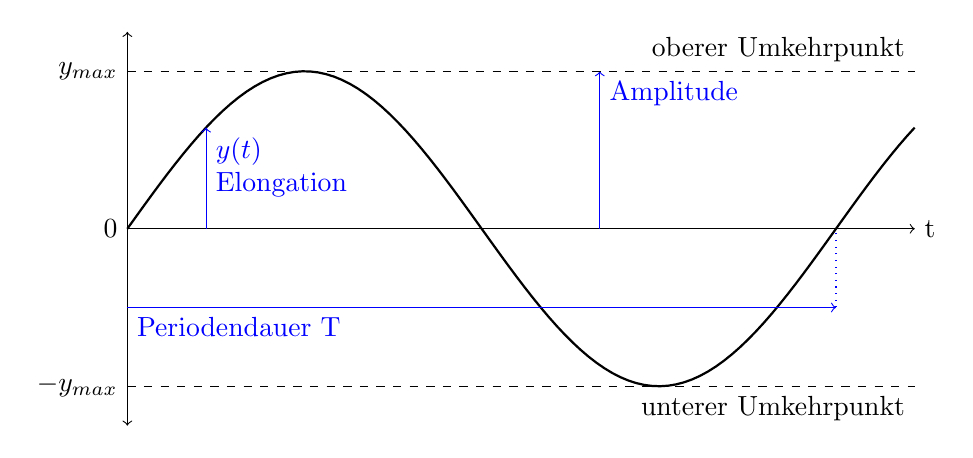
\begin{tikzpicture}     
  \draw[thick, domain=0:10, samples=100] 
            plot (\x, {2*sin(\x*360 / 9)});
     
  \draw[->] (0, 0) -- (10, 0) node[right] {t};
  
  \draw (0, 0) node[left] {$0$}; 
  \draw (0, 2) node[left] {$y_{max}$}; 
  \draw (0, -2) node[left] {$-y_{max}$};
  \draw[<->] (0, -2.5) -- (0, 2.5); 
  
  \draw[->, blue] (1, 0) -- (1, {2*sin(1*360/9)}) node[below right, align=left] {$y(t)$ \\ Elongation};  
  \draw[->, blue] (6, 0) -- (6, 2) node[below right] {Amplitude};  
  \draw[->, blue] (0, -1) node[below right] {Periodendauer T} -- (9, -1);
  \draw[dotted, blue] (9, -1) -- (9, 0);
 
  \draw[dashed] (0, 2) -- (10, 2) node[above left] {oberer Umkehrpunkt};
  \draw[dashed] (0, -2) -- (10, -2) node[below left] {unterer Umkehrpunkt};  
 \end{tikzpicture}
\end{figure} 
 
\noindent Schwingungsfrequenz $f=\frac{1}{T}=\frac{n}{t}$, offensichtlich
 
\subsection*{Bogenmaß}
\[ 
 \varphi = \frac{b}{r}
\quad \text{und} \quad 
 360^\circ = 2\pi
\]
 
\subsection*{Schwingungsgleichung}
\[
 y(t)=y_{max} \cdot \sin{\omega \cdot t}
\quad \text{und} \quad 
 y(t)=y_{max} \cdot \sin{\frac{2\pi}{T} \cdot t}
\]
 
\subsection*{Federoszilator}
Mit der Federkonstante bzw. Federhärte $D$ in $\dfrac{\text{Newton}}{\text{Meter}}$ gilt
\[
 F = D \cdot \Delta y
\]
 
\subsubsection*{Schwingungsdauer}
Zu jedem Zeitpunkt setzt sich $F=Dy$ das Grundgesetz $F=ma$ gleich groß entgegen, sodass
\[
 D \cdot y + m \cdot a = 0
\]
Wird dann die Schwingungsgleichung und dessen zweite Ableitung als $y$ und $a$ und $\omega = \frac{2\pi}{T}$ eingesetzt und etwas umgeformt, vereinfacht durch den Satz vom Nullprodukt, findet man
\[
 T = 2\pi \cdot \frac{\sqrt{m}}{\sqrt{D}} 
\]  
 
\subsubsection*{Horizontal}
Bei einem horizontalen Federoszilator, bei welchem zwei gegenüberliegenden Federn an einem mit Rädern frei bewegbaren Wagen befestigt sind, zeigt als $D$ des gesamten Federoszilators die Summe der $D$s der zwei einzelnen Federn auf.  
 
\subsection*{Kleinwinkelnäherungen}
Bei kleinen Winkeln als RAD gilt $x \approx \sin x$ und $x \approx \tan x$. Bis $7^\circ$ ist die Abweichung $< 0.25\%$
 
\section{Definition}
Eine Schwingung ist eine zeitlich periodische Veränderung einer physikalischen Größe. Nach einmaliger Auslenkung aus der Ruhelage treten rücktreibene Kräft ein. \newline
Eine Schwingung ist eine harmonische Schwingung, wenn
\begin{enumerate}
 \item sie mit einer Sinusfunktion beschrieben werden kann
 \item sie auf eine gleichförmige Kreisbewegung zurückgeführt werden kann
 \item die Schwingungsdauer zeitlich konstant ist
 \item die Rücktreibene Kraft zur Elongation proportional ist 
\end{enumerate}  
Diese Aussagen sind äquivalent zueinander; wenn eine Stimmt, stimmen alle. 
 
\section{Bogenmaß}
In einem Bogen mit dem Radious $r$ und dem Bogenlänge $b$ gilt 
\[
 \varphi = \frac{b}{r} 
\]
Für einen vollen Kreis, eigentlich einem Bogen mit einem Winkel vom $360^\circ$, ist die Bogenlänge der Umfang $U=2 \pi r$, sodass die $r$s wegfallen und
\[
 360^\circ = 2\pi
\]
  
\section{Schwingungsgleichung}
Einer gleichförmigen Kreisbewegung nach ist, bei welcher die Höhe bei $0$ started, folgt die Höhe einer Sinusfunktion, welche zu $y_{max}$ geht, also
\[
 y(t)=y_{max} \cdot \sin{\varphi}
\]
mit der Winkelgeschwindigkeit als $\omega = \dfrac{\varphi}{t}$ gilt dann die Schwingungsgleichung
\[
 \boxed{y(t)=y_{max} \cdot \sin{\omega \cdot t}}
\]
bzw. für eine komplette Periode mit der Periodendauer $T$ mit dem Bogenmaß $360^\circ = 2\pi$ gilt
\[
 \boxed{y(t)=y_{max} \cdot \sin{\frac{2\pi}{T} \cdot t}} 
\]
 
\section{Federoszilator}
Das Hookesche Gesetz besagt, dass die wirkenen Kraft eines Federoszilators zur Längenänderung propotional ist, sodass
\[
 F = D \cdot \Delta y
\]
mit der Federkonstante bzw. Federhärte $D$ in $\dfrac{\text{Newton}}{\text{Meter}}$
 
\subsection{Schwingungsdauer}
Zu jedem Zeitpunkt setzt sich $F=Dy$ das Grundgesetz $F=ma$ gleich groß entgegen, sodass
\begin{equation}
 D \cdot y + m \cdot a = 0
\end{equation}
Dabei ist die Schwingungsgleichen $y$ und dessen zweiten Ableitung als $a$
\begin{align}
y(t)&=y_{max} \cdot \sin{\omega \cdot t} \\
a(t)&=-y_{max} \cdot \omega^2 \cdot \sin{\omega \cdot t}
\end{align} 
Eingesetzt gilt dann 
\begin{equation}
 D \cdot y_{max} \cdot \sin{(\omega \cdot t)} - m \cdot y_{max} \cdot \omega^2 \cdot \sin{(\omega \cdot t)} = 0
\end{equation} 
Das $y_{max}$ und $\sin{\omega t}$ kann dann ausgeklammert werden zu \begin{equation}
 y_{max} \cdot \sin{\omega t} \cdot (D - m \cdot \omega^2) = 0 
\end{equation} 
Mit dem Satz vom Nullprodukt können alle Faktoren, welche nicht permament Null sein können ignoriert werden, sodass nur $D - m \cdot \omega^2 = 0$ relevant ist. \newline
Um $T$ zu finden muss nurnoch die Winkegeschwindigkeit $\omega = \dfrac{2\pi}{T}$ eingesetzt werden. Beim weiteren Umformen ist $\sqrt{a}\cdot\sqrt{b}=\sqrt{a \cdot b}$ hilfreich. 
Es folgt 
\begin{equation}
 T = 2\pi \cdot \frac{\sqrt{m}}{\sqrt{D}}
\end{equation} 
So kann dann wenn $T=k \cdot \sqrt{m}$ gegeben ist $k=\dfrac{2\pi}{\sqrt{D}}$ nach D aufgelöst werden. 
 
\section{Fadenpendel}
\begin{wrapfigure}{r}{4cm}
 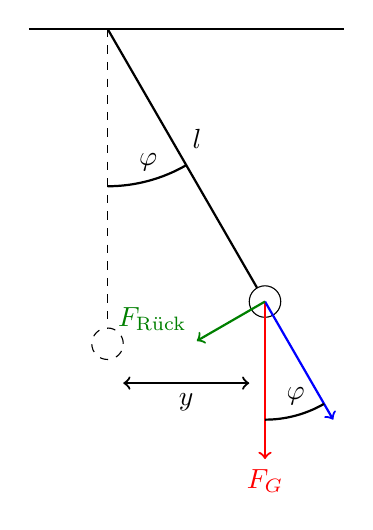
\begin{tikzpicture}
  \draw[thick] (-1, 0) -- (3, 0);
  \draw[dashed] (0, 0) -- (0, -3.8);
  \draw[dashed] (0, -4) circle (0.2);
  \draw[thick] (0, 0) -- ({3.8*sin(30)}, {-3.8*cos(30)}) node[midway,above right] {$l$};
  \draw ({4*sin(30)}, {-4*cos(30)}) circle (0.2);
 
  \draw[thick] (0, -2) arc[start angle=270,end angle=300,radius=2] node[midway, above] {$\varphi$};
  
  \draw[->,thick,red] ({4*sin(30)}, {-4*cos(30)}) -- ++(0, -2) node[below] {$F_G$};
  \draw[->,thick,blue] ({4*sin(30)}, {-4*cos(30)}) -- ++({2*cos(30)*sin(30)}, {-2*cos(30)*cos(30)});
 
  \draw[thick] ({4*sin(30)}, {-4*cos(30)-1.5}) arc[start angle=270,end angle=300,radius=1.5] node[midway, above] {$\varphi$};
 
  \draw[->,thick,green!50!black] ({4*sin(30)}, {-4*cos(-30)}) -- ++({2*cos(60)*sin(-60)}, {-2*cos(60)*cos(-60)}) node[above left] {$F_{\text{Rück}}$};
 
  \draw[<->, thick] (0.2, -4.5) -- (1.8, -4.5) node [midway, below] {$y$};  
 \end{tikzpicture}
\end{wrapfigure}
 
\setcounter{equation}{0} 
Die Gewichtskraft $F_G$ teilt sich auf in einen Anteil der am Faden zeiht und einen Teil der den Körper in Richtung der Ruhelage bewegen "will". \newline
Dabei ist
\begin{equation}
 \sin \varphi = \frac{F_{\text{Rück}}}{F_G}
\end{equation} 
umgestellt nach
\begin{equation}
 F_{\text{Rück}} = m \cdot g \cdot \sin{\varphi}
\end{equation}  
Wobei der Kleinwinkelnäherungen nach für kleinere Winkel $\varphi = \sin{\varphi}$, weshalb 
\begin{equation} 
 F_{\text{Rück}} = m \cdot g \cdot \varphi
\end{equation}  
Mit $\tan \varphi = \dfrac{y}{l}$ 
\begin{equation} 
 F_{\text{Rück}} = \frac{m \cdot g}{l} \cdot y
\end{equation}
Somit ist $F_{\text{Rück}}$ zu $y$ proportional und Fadenpendel zeigt eien harmonische Schwingung auf. Ähnlich wie bei der Herleitung der Schwingungsdauer des Federoszilators kann hier die
\[
 F_{\text{Rück}} + m \cdot a = 0
\]
gesetzt werden um die Schwingungsdauer herzuleiten und am Ende auf
\[
 T = 2\pi \cdot \sqrt{\frac{l}{g}} 
\] 
 
\section{Messunsicherheiten}
Der experimentell bestimmte Wert kann nicht genauer sein, als der Messwert mit den größten Messunsicherheit. Misst man den Wert $x$ der Größe $G$ und geht von der unsicherheit $u$ aus (als Dezimalzahl), dann ist
\[
 G = x \pm x \cdot u
\]
bzw. 
\[
 x - x \cdot u < G < x + x \cdot u
\]
Wird beispeilsweise die Federkonstante $D=5 \frac{\si{\newton}}{\si{\meter}}$ gemessen, wobei der Messwerte um $10\%$ falsch liegen könnt, weil beiden Messungen $10$ Sekunden mit einer Reaktionsgeschwindigkeit von $1$ Sekunde gemessen wurden, ist
\[
 D = 5 \frac{\si{\newton}}{\si{\meter}} \pm 0.5 \frac{\si{\newton}}{\si{\meter}}
\] 
bzw.
\[
 4.5 \frac{\si{\newton}}{\si{\meter}} < D < 5.5 \frac{\si{\newton}}{\si{\meter}}
\] 
 
\end{document}
 
 
 
 
 
